\documentclass{article} 

\usepackage{amsmath} 

\title{Trabajo practico computacional} 
\author{Franco, Lautaro, Nicol\'as, Tomas}
\date{\today}

\usepackage{graphicx}
\graphicspath{ {./figures/} }

\renewcommand{\theenumi}{\alph{enumi}}
\begin{document}
    \maketitle
    
    \section{DCL}
    
    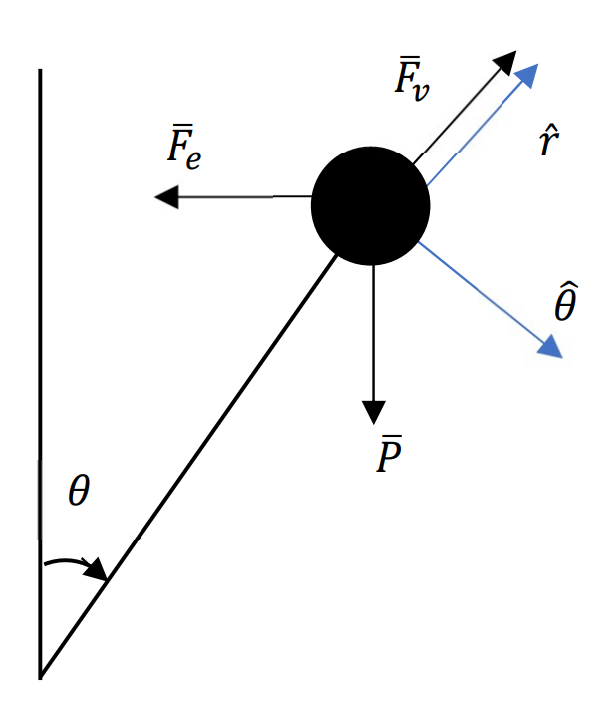
\includegraphics[scale=0.3]{DCL.png}
    
    \section{Ecuaciones de Newton}
    
    En base al diagrama de cuerpo libre definimos las fuerzas peso y el\'astica de la siguiente forma:
    
	$$\vec{F}_e = kR \sin^2{(\theta)} \hat{r} + kR \sin{(\theta)}\cos{(\theta)} \hat{\theta}$$
	$$\vec{P} = -mg \cos{(\theta)} \hat{r} + mg \sin {(\theta)} \hat{\theta} $$
	
	Desarrollamos las ecuaciones de Newton:
	
	\begin{equation}
	\label{eqn:equationr}
		\hat{r)} \quad -mR\dot{\theta}^2 = F_v - mg \cos{(\theta)} - kR \sin^2{(\theta)}
	\end{equation}
    
    \begin{equation}
    \label{eqn:equationtheta}
    	\hat{\theta}) \quad mR\ddot{\theta} = mg \sin{(\theta)} - kR \sin{(\theta)} \cos{(\theta})
    \end{equation}
    
    \section{Fuerza de v\'inculo}
    
    Para trabajar $F_v(\theta)$, trabajaremos con la ecuaci\'on de movimiento
    
    $$mR\ddot{\theta} = mg \sin{(\theta)} - kR \sin{(\theta)} \cos{(\theta)}$$
    $$\ddot{\theta} = \frac{g}{R} \sin{(\theta)} - \frac{k}{m} \sin{(\theta)} \cos{(\theta)}$$
   	Utilizando regla de la cadena,
   	
   	 $$ \int_{\dot{\theta}_0 = 0 \frac{\textbf{rad}}{\textbf{s}}}^{\dot{\theta}} \! \dot{\theta} \, d\dot{\theta} =
   	 	\int_{\theta_0}^{\theta} \! \frac{g}{R} \sin{(\theta)} \, d\theta -
   	 	\int_{\theta_0}^{\theta} \! \frac{k}{m} \sin{(\theta)} \cos{(\theta)} \, d\theta$$
   	 	
   	 $$ \frac{\dot{\theta}^2}{2} =
   	 	-\frac{g}{R} [ \cos{\theta} - \cos{(\frac{\pi}{2})} ] - \frac{k}{2m}(\sin^2{\theta} - 1) $$
   	 	
   	 $$ \dot{\theta}^2 =
   	 	-2\frac{g}{R} [ \cos{\theta} - \cos{(\frac{\pi}{2})} ] - \frac{k}{m}(\sin^2{\theta} - 1) $$
   	 	
   	 Una vez obtenida esta ecuaci\'on, metemos en (\ref{eqn:equationr}) para as\'i poder despejar $F_v(\theta)$. Queda:
   	 
   	 $$
   	 -mR[-2\frac{g}{R} [ \cos{(\theta)} - \cos{(\frac{\pi}{2})} ] - \frac{k}{m}(\sin^2{(\theta)} - 1)] = F_v - mg \cos{((\theta))} - kR \sin^2{(\theta)}
   	 $$
   	 
   	 $$
   	 	2mg \cos{(\theta)} + kR(\sin^2{(\theta)} - 1) = F_v - mg\cos{(\theta)} + kR\sin^2{(\theta)}
   	 $$
   	 
   	 $$
   		3mg \cos{(\theta)} - 2kR\sin^2{(\theta)} - kR = F_v
   	 $$
   	 
   	 Para hallar los puntos de equilibrio anal\'iticamente, pedimos $f(\theta) = 0$. En (\ref{eqn:equationtheta}), si $mR \ddot{\theta} = f(\theta) = 0 \textbf{N}$, hay equilibrio. De (\ref{eqn:equationtheta}):
   	 
   	 
   	$$
   	\quad mR\ddot{\theta} = mg \sin{(\theta)} - kR \sin{(\theta)} \cos{(\theta)})
   	$$
   	 
   	$$
   	0 = \sin{(\theta_{\textbf{eq}})} (mg - kR \cos{(\theta_{\textbf{eq}})})
   	$$
   	 
   	Entonces,
   	 
   	 $$\rightarrow \sin{\theta_{\textbf{eq}}} = 0 \rightarrow \theta_{\textbf{eq}} \in \lbrace 0, \pi \rbrace $$
   	 
   	O bien,
   	 
   	$$
		mg - kR \cos{(\theta_{\textbf{eq}})} = 0 
	$$
	$$
		\leftrightarrow mg = kR \cos{(\theta_{\textbf{eq}})} 
   	$$
   	$$
		\leftrightarrow \arccos{\frac{mg}{kR}} = \arccos{\cos{(\theta_{\textbf{eq}})}} 
   	$$
   	$$
		\rightarrow \theta_{\textbf{eq}} \in \lbrace \arccos{(\frac{mg}{kR})}, -\arccos{(\frac{mg}{kR})} \rbrace 
   	$$

	Hallamos, los siguientes puntos de equilibrio:
	
	$$\theta_{\textbf{eq}} \in \lbrace 0, \pi, \pm1.37 \rbrace \textbf{rad}$$
	
	Siendo consistentes con los puntos de equilibrio hallados en el problema 4.9. En cuanto a su estabilidad, buscamos $f'(\theta)$ y la evaluamos en los puntos de equilibrio encontrados. Analizamos su signos.
	
	$$
		f'(\theta) = \cos{(\theta)} (\frac{g}{R} - \frac{k}{m} \cos{\theta}) + \sin{\theta} \sin{\theta} \frac{k}{m}  
	$$
	$$
		\leftrightarrow f'(\theta) = \cos{(\theta)} (\frac{g}{R} - \frac{k}{m} \cos{\theta}) + \sin^2 {\theta} \frac{k}{m}  
	$$
	
	Reemplazando:
	
	$$f'(0) < 0 \rightarrow \textsf{Estable}$$
	$$f'(\pi) < 0 \rightarrow \textsf{Estable}$$
	$$f'(\pm \arccos{(\frac{gm}{Rk})}) > 0 \rightarrow \textsf{Inestable}$$
	
	Coincidiendo con lo pedido, determinando $\theta = 0$ como estable, debido a que $\frac{g}{R} < \frac{k}{m}$

	Luego al comparar con la aproximaci\'on num\'erica graficada con Python, obtuvimos que las ra\'ices (marcadas con puntos) coinciden, con un error despreciable de la soluci\'on anal\'itica.
		
	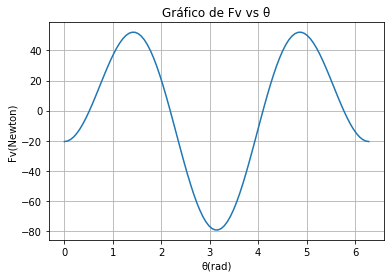
\includegraphics[scale=0.5]{01.png}
	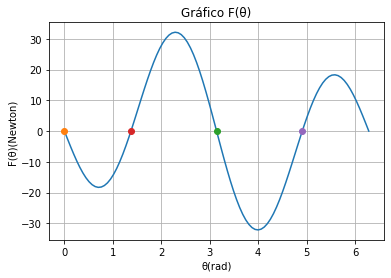
\includegraphics[scale=0.5]{02.png}

	\section{Pequeñas oscilaciones vs. soluci\'on num\'erica}
	
	Para buscar la soluci\'on anal\'itica utilizaremos pqueñas oscilaciones. Para ello, desarrollamos el polinomio de Taylor de orden 1 de $f(\theta)$ en un entorno a $\theta_{\textbf{eq}} = 0$.
	
	$$
		f(\theta) \simeq f(\theta_{\textbf{eq}}) + f'((\theta_{\textbf{eq}}))(\theta - \theta_{\textbf{eq}})
	$$
	\begin{equation}
	\label{eqn:taylor}
		f(\theta) \simeq (\cos{\theta_{\textbf{eq}}}(\frac{g}{R} - \frac{k}{m}\cos(\theta_{\textbf{eq}})) + \sin^2{(\theta)})(\theta - \theta_{\textbf{eq}})
	\end{equation}
	
	$$f(0) \simeq (\frac{g}{R} - \frac{k}{m})\theta$$
	
	Para que tenga sentido fisica, $\frac{g}{R} < \frac{k}{m}$ porque sino ser\'ia un equilibrio inestable y no podr\'ia oscilar. Entonces, coincide con la resoluci\'on num\'erica.
	
	\begin{enumerate}
		\item Estos resultados tienen sentido f\'isico ya que al posicionar la masa en el punto de equilibrio 0 el resorte crea una mayor fuerza (el\'astica) que el peso ($kR > mg$), y en $\pi$ ambas fuerzas "trabajan en conjunto" restituyendo a la masa a su posici\'on de equilibrio luego de un corrimiento de la misma. Luego, los puntos $\pm 1.37$ que provienen de la ecuacion (\ref{eqn:equationtheta}) aparentemente tambi\'en coinciden con el gr\'afico y son posibles debido a que $mg<kR$ ya que la funci\'on $\arccos{}$ tiene el dominio limitado tal que $\theta \in [-1;1] \textbf{rad}$.
		
		\item Luego de aproximar la ecuaci\'on de movimiento para peque\~nas oscilaciones obtenemos la ecuaci\'on (\ref{eqn:taylor}), y despejamos $\omega$ resultando:
		
		\begin{equation}
		\label{omega}
			\omega = \pm\sqrt{mg - kR}
		\end{equation}
		
		Para que tenga sentido f\'isico se debe respetar que $\frac{g}{R} < \frac{k}{m}$ ya que solo as\'i el punto de equilibrio puede ser estable y por ende oscilar (sino no tendr\'ia sentido hablar de peque\~nas oscilaciones). En cuanto a $\dot{\theta}_i$, debemos considerar un intervalo el cual llegue hasta el punto l\'imite donde la velocidad inicial causa que la masa "salga" definivamente del punto de equilibrio y deje de oscilar. Finalmente, $\dot{\theta}_i \in [0;5.7] \frac{\textbf{rad}}{\textbf{s}}$.
		
		\item Luego proponemos una soluci\'on a la ecuaci\'on diferencial mediante la ecuaci\'on:
		
		\begin{equation}
		\label{coseno}
			\theta(t) = A \cos{\omega t + \phi}
		\end{equation}
		
		Resulta, de (\ref{coseno}), resulta
			$$\dot{\theta}(t) = -A \omega \sin{\omega t + \phi}$$
			
		y con las condiciones iniciales dadas por el enunciado, obtenemos la amplitud $A$ y la fase $\phi$. Al graficar este resultado y compararlo con el m\'etodo num\'erico realizado con \emph{odeint} podemos sacar las siguientes conclusiones: Nos encontramos con que las funciones acuerdan con un error despreciable, siendo practicamente iguales ($\dot{\theta}_i = 0.1 \frac{\textbf{rad}}{\textbf{s}}$).
		
		
		
		Para $\dot{\theta}_i = 3 \frac{\textbf{rad}}{\textbf{s}}$ notamos un desfase marcado, que con el paso del tiempo va aumentando.
		
		
		
		Para $\dot{\theta}_i = 10 \frac{\textbf{rad}}{\textbf{s}}$ notamos un gr\'afico diferente a los que ven\'iamos teniendo. Nos encontramos ante una situaci\'on en la cual la velocidad inicial es tan alta que deja de haber oscilaci\'on, dado que la masa \emph{sale} del punto de equilibrio.
		
		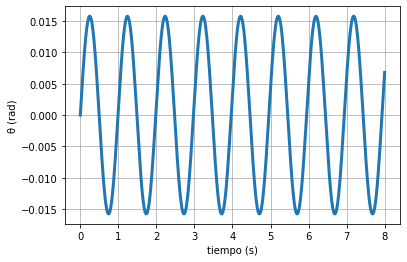
\includegraphics[scale=0.5]{03.png}
		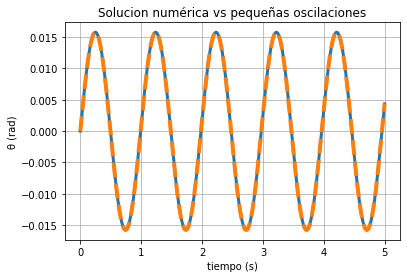
\includegraphics[scale=0.5]{04.png}
		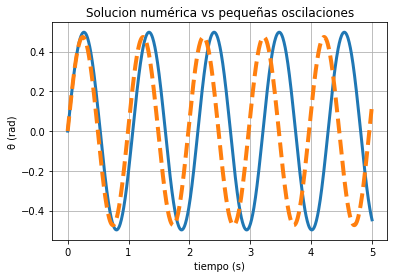
\includegraphics[scale=0.5]{05.png}
		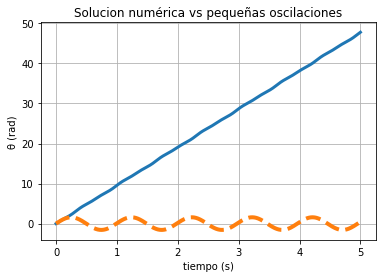
\includegraphics[scale=0.5]{06.png}
		
		\item Cambiando el valor de $k$ por $k = 5 \frac{\textbf{N}}{\textbf{m}}$ no nos encontramos, claramente, con el comportamiento t\'ipico de peque\~as oscilaciones dado que no hay oscilaci\'on. Como $k = 5 \frac{\textbf{N}}{\textbf{m}}$ tenemos que en $\theta = 0$ hay un equilibrio inestable, ya que $\frac{g}{R} > \frac{k}{m}$.
		
		
		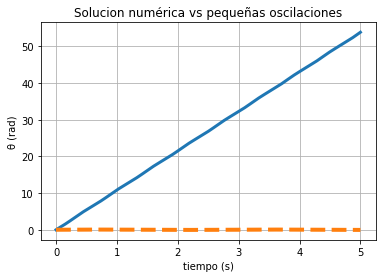
\includegraphics[scale=0.5]{07.png}
		
		Al analizar los gr\'aficos podemos ver que para $t \in [0,2)$ hay un acuerdo entre ambas soluciones. Luego de $t=2\textbf{s}$ comienza a haber un desfase y con el paso del tiempo el desfase aumenta notablemente. En cuanto a la posicion angular, notemos que cuando $\theta$ es muy peque\~na, los gr\'aficos coinciden. Incluso encontramos acuerdo hasta $\theta \simeq 1 \textbf{rad}$. Luego empieza el desfase y con el tiempo aumenta.
			
	\end{enumerate}
	
\end{document}